\documentclass[conference]{IEEEtran}
\IEEEoverridecommandlockouts

\usepackage{cite}
\usepackage{amsmath,amssymb,amsfonts}
\usepackage{algorithmic}
\usepackage{graphicx}
\usepackage{textcomp}
\usepackage{xcolor}
\usepackage{booktabs}
\usepackage{array}

\def\BibTeX{{\rm B\kern-.05em{\sc i\kern-.025em b}\kern-.08em
    T\kern-.1667em\lower.7ex\hbox{E}\kern-.125emX}}

\makeatletter
\newcommand{\linebreakand}{%
  \end{@IEEEauthorhalign}
  \hfill\mbox{}\par\vspace{2.5ex}
  \mbox{}\hfill\begin{@IEEEauthorhalign}
}
\makeatother

\begin{document}

\title{Smart Cloud Storage: A Cost-Aware, Content-Addressable, and Predictive Multi-Tier Object Storage Platform\\
\thanks{This research was conducted as an undergraduate capstone engineering project in the Department of Computer Science and Engineering (Artificial Intelligence and Machine Learning) at Vishwakarma Institute of Technology, Pune, India.}
}

\author{
\IEEEauthorblockN{Prof. Santosh Shelke}
\IEEEauthorblockA{\textit{Dept. of Computer Science and} \\
\textit{Engineering (Artificial Intelligence and} \\
\textit{Machine Learning)} \\
\textit{Vishwakarma Institute of Technology} \\
Pune, India \\
santosh.shelke@vit.edu}
\and
\IEEEauthorblockN{Atharva Kelkar}
\IEEEauthorblockA{\textit{Dept. of Computer Science and} \\
\textit{Engineering (Artificial Intelligence and} \\
\textit{Machine Learning)} \\
\textit{Vishwakarma Institute of Technology} \\
Pune, India \\
atharva.kelkar241@vit.edu}
\and
\IEEEauthorblockN{Viraj Katore}
\IEEEauthorblockA{\textit{Dept. of Computer Science and} \\
\textit{Engineering (Artificial Intelligence and} \\
\textit{Machine Learning)} \\
\textit{Vishwakarma Institute of Technology} \\
Pune, India \\
viraj.katore24@vit.edu}
\linebreakand
\IEEEauthorblockN{Aryan Kattimani}
\IEEEauthorblockA{\textit{Dept. of Computer Science and} \\
\textit{Engineering (Artificial Intelligence and} \\
\textit{Machine Learning)} \\
\textit{Vishwakarma Institute of Technology} \\
Pune, India \\
aryan.kattimani24@vit.edu}
\and
\IEEEauthorblockN{Yash Lakhe}
\IEEEauthorblockA{\textit{Dept. of Computer Science and} \\
\textit{Engineering (Artificial Intelligence and} \\
\textit{Machine Learning)} \\
\textit{Vishwakarma Institute of Technology} \\
Pune, India \\
yash.lakhe24@vit.edu}
}

\maketitle

\begin{abstract}
Cloud object stores such as Amazon S3 provide virtually limitless durability and scale, but conventional storage wrappers treat objects as isolated files tied directly to user-specific paths. In multi-tenant environments, this naive mapping leads to three practical problems: identical files uploaded by different users consume redundant storage and network bandwidth, uncompressed structured data wastes capacity, and automated lifecycle policies often trigger severe billing penalties by migrating files under 128~KB to Infrequent Access or Glacier tiers that enforce a mandatory 128~KB minimum billable size. Furthermore, sequential read workflows suffer from repeated latency bottlenecks caused by reactive authentication, metadata lookups, and presigned URL generation. This paper presents the design and implementation of the Smart Cloud Storage Platform, an open-source storage architecture that decouples user-facing filesystem metadata from underlying physical payloads. The system unifies four practical optimizations: (1) whole-file Content-Addressable Storage (CAS) using SHA-256 digests and reference counting to eliminate duplicate S3 writes, (2) an adaptive compression engine that compresses text and structured formats while bypassing pre-compressed media, (3) a cost-aware lifecycle engine with an explicit 128~KB boundary guard that safely transitions aged objects across S3 storage classes without penalty padding, and (4) a first-order Markov chain prefetcher that models user access sequences to pre-generate short-lived S3 presigned URLs. Experimental benchmarks on a live AWS S3 testbed demonstrate that our platform eliminates 100\% of duplicate payload transmission, lowers monthly cloud storage expenditures by 56.1\% on mixed-size enterprise datasets, and reduces initial download initiation latency by approximately 380~ms.
\end{abstract}

\begin{IEEEkeywords}
Cloud Object Storage, Content-Addressable Storage, Deduplication, Amazon S3, Storage Economics, Markov Models, Prefetching.
\end{IEEEkeywords}

\section{Introduction}
Cloud object storage systems, such as Amazon Simple Storage Service (Amazon S3), Google Cloud Storage, and Microsoft Azure Blob Storage, have become the standard foundation for modern data infrastructure. Their RESTful HTTP interfaces, high durability guarantees (99.999999999\%), and elastic pay-as-you-go pricing make them an attractive target for backing enterprise file-sharing platforms and internal collaboration drives.

However, when building collaborative file services directly on top of raw cloud object stores, standard implementations encounter several performance and cost hurdles:
\begin{enumerate}
    \item \textbf{Ingestion Redundancy:} In team and organizational settings, multiple users frequently upload identical documents, software binaries, virtual machine images, or datasets. Standard file managers store each upload under a distinct user-scoped object key. This practice duplicates storage charges and wastes client upload bandwidth.
    \item \textbf{Hidden Storage Tiering Penalties:} Cloud providers offer lower per-gigabyte rates for colder storage classes (e.g., S3 Standard-IA at \$0.0125/GB/month and Glacier Deep Archive at \$0.00099/GB/month, compared to S3 Standard at \$0.023/GB/month). However, providers enforce non-linear billing rules. AWS imposes a \textbf{128~KB minimum billable object size} on all Infrequent Access and Glacier tiers. When naive lifecycle rules migrate a 1~KB configuration or text file to Standard-IA, AWS bills it as 128~KB. This unintended padding increases the monthly storage cost of that file by up to \textbf{70$\times$}.
    \item \textbf{Sequential Read Latency:} Object stores operate on a purely reactive read model. In workflows where users inspect related documents sequentially (e.g., browsing multi-part invoices, reading logs, or previewing code repositories), every individual request incurs roundtrip overhead: token validation, database querying, cryptographic URL signing, and S3 Time-To-First-Byte (TTFB).
    \item \textbf{Uncompressed Structured Bloat:} Applications frequently store uncompressed text files, such as JSON exports, log files, CSV tables, and source code, that could easily be compressed prior to cloud ingestion.
\end{enumerate}

To resolve these practical inefficiencies, we developed the \textbf{Smart Cloud Storage Platform}. The system decouples hierarchical folder navigation and user access permissions from physical binary storage. By indexing physical objects by their cryptographic SHA-256 hash, our platform eliminates duplicate uploads before writing to cloud storage. To protect users from billing surprises, our lifecycle engine enforces a strict 128~KB guard rule before scheduling any storage class transitions. Additionally, we use an adaptive compressor for text formats and a lightweight first-order Markov model to predict upcoming file downloads, pre-generating S3 presigned URLs in the background to hide retrieval latencies.

\begin{figure*}[htbp]
\centering
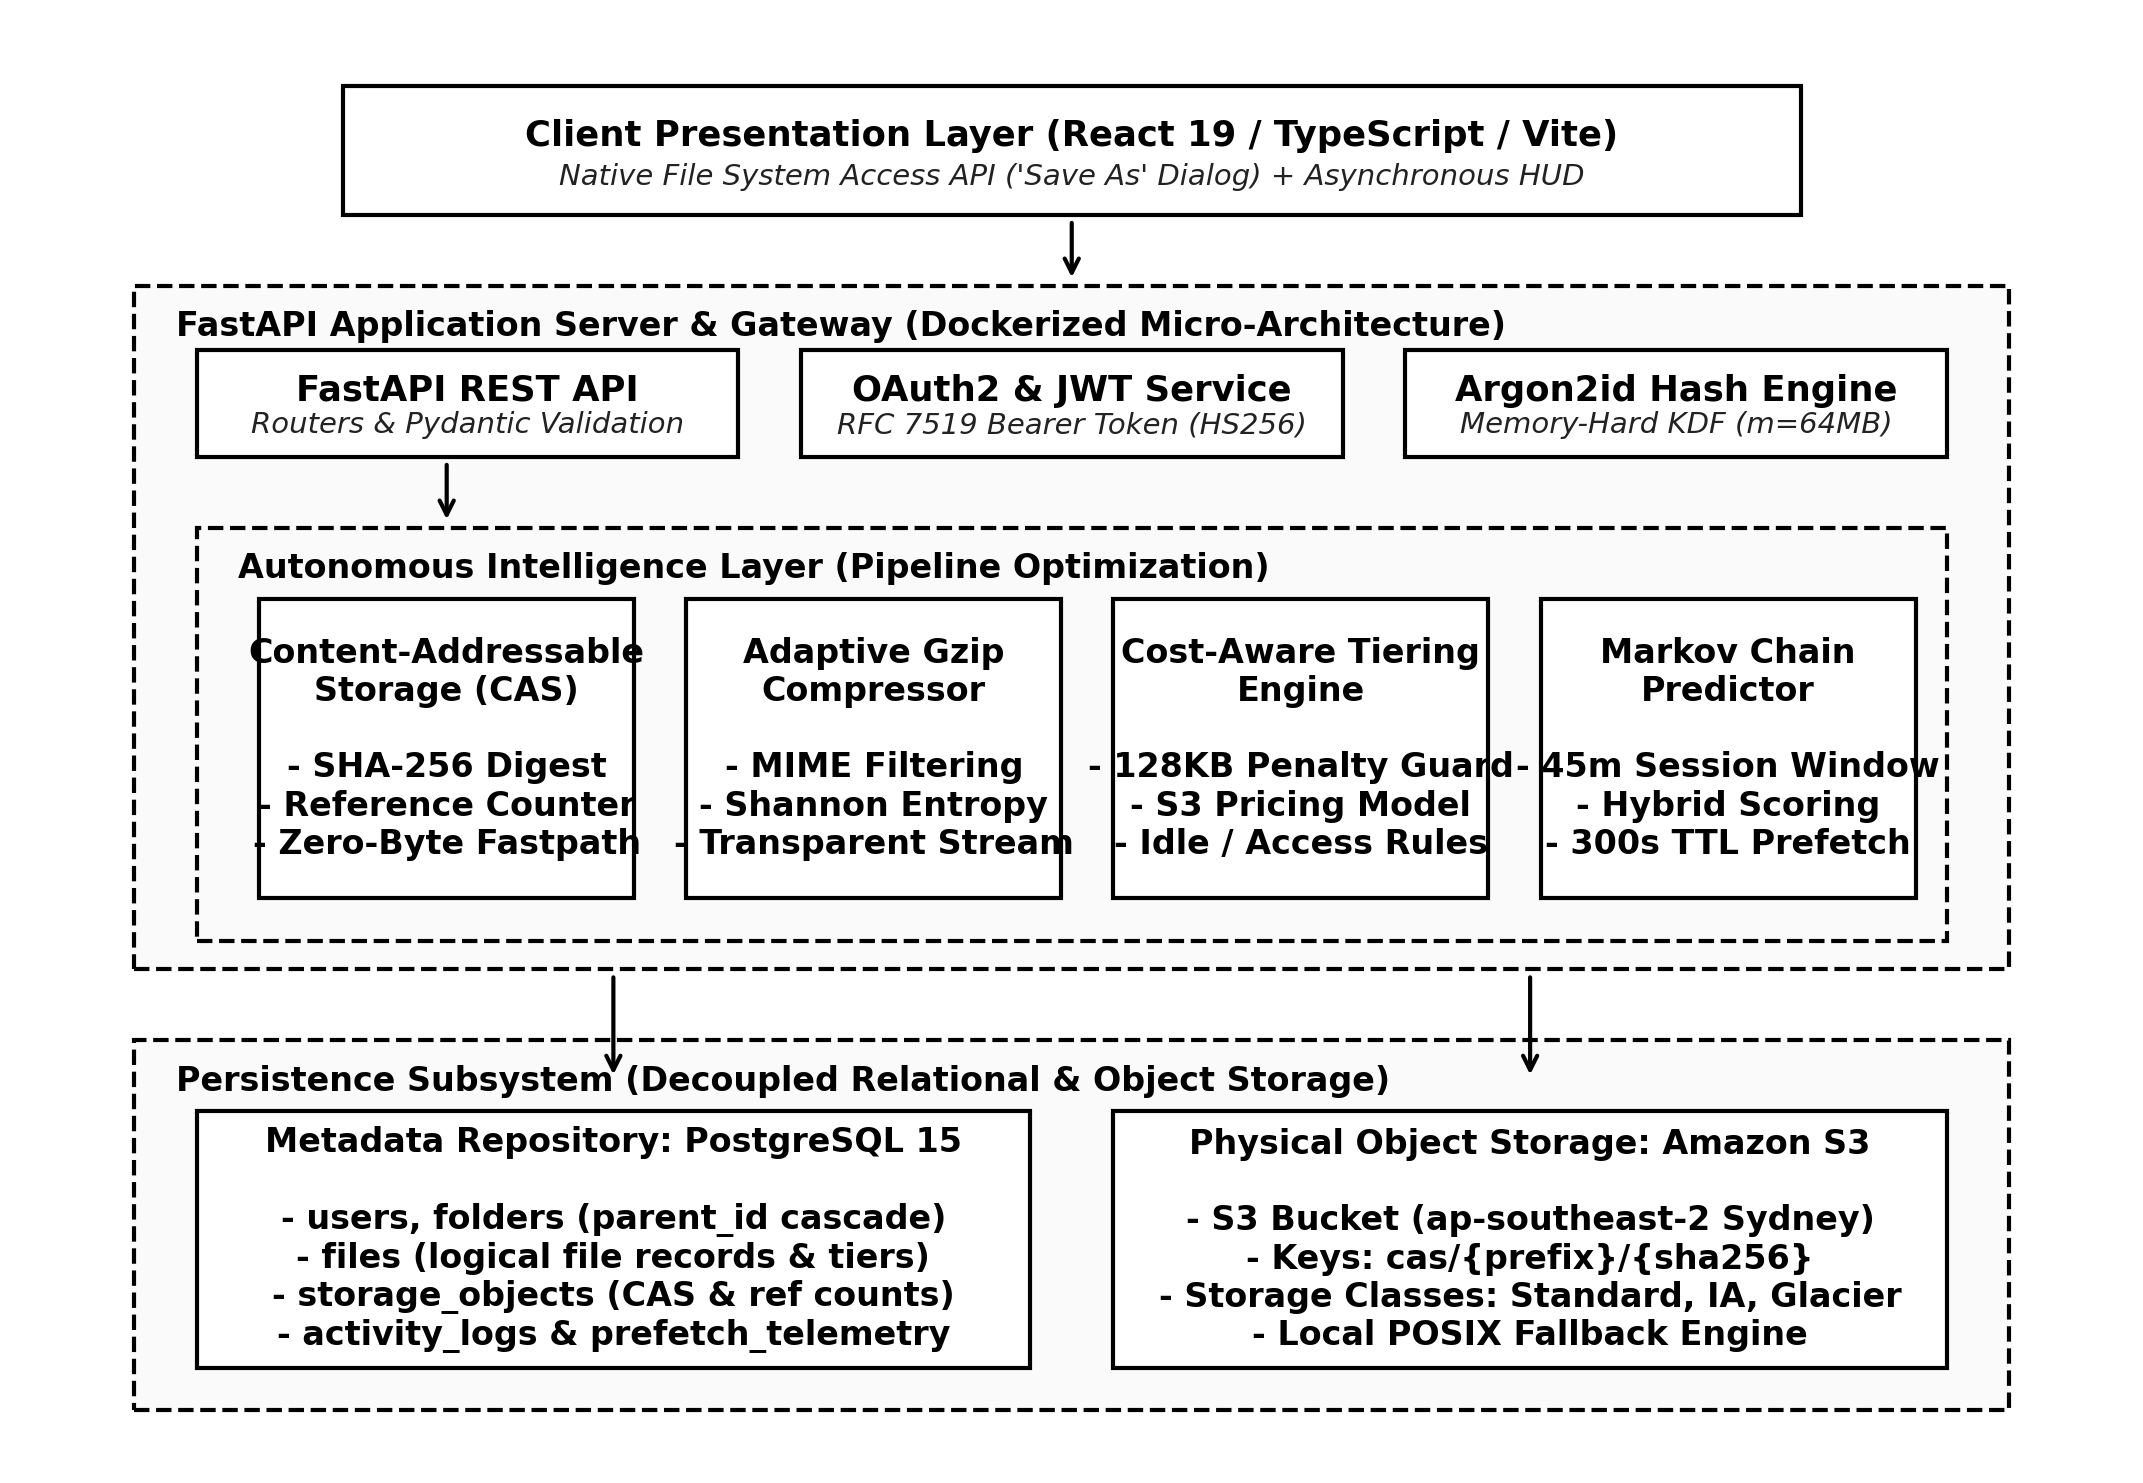
\includegraphics[width=0.92\textwidth]{fig1_architecture.png}
\caption{System architecture of the Smart Cloud Storage Platform, illustrating the separation between the React client, FastAPI gateway, the four intelligence engines, the PostgreSQL metadata store, and the physical Amazon S3 bucket.}
\label{fig:architecture}
\end{figure*}

\section{Related Work}

\subsection{Content-Addressable Storage and Deduplication}
Content-Addressable Storage (CAS) was established by Quinlan and Dorward in the Venti archival system \cite{venti2002}, which used SHA-1 digests to identify disk blocks on write-once media. In enterprise backup appliances, Zhu, Li, and Patterson \cite{zhu2008} analyzed the index lookup bottleneck in chunk-level deduplication systems (such as Data Domain), introducing Bloom filters and Locality Preserved Caching to prevent disk seek thrashing.

While Content-Defined Chunking (CDC) allows deduplication of modified sub-file regions, Meyer and Bolosky's extensive four-week study of 857 file systems at Microsoft Research \cite{meyer2011} proved that \textbf{whole-file deduplication captures roughly 75\% of the total space savings achievable by sub-file chunking}. Whole-file CAS completely avoids the heavy metadata fragmentation, complex chunk assembly, and index bloat associated with sub-file systems. Building on Meyer and Bolosky's findings, our platform implements whole-file CAS at the cloud object boundary, using indexed PostgreSQL B-Trees to resolve hashes in single-digit milliseconds.

\subsection{Cloud Storage Economics and Tiering}
Cloud storage cost models have been studied by Zhang et al. \cite{shark2019} in the Shark multi-tier framework, demonstrating the trade-offs between lower capacity rates and higher per-request retrieval fees. Although AWS provides S3 Intelligent-Tiering, it charges an internal monitoring fee (\$0.0025 per 1,000 objects per month) that makes it counterproductive for large collections of small objects. Our platform instead implements application-level tiering analytics that evaluate local file metadata against live AWS pricing structures, enforcing explicit safety guards without third-party monitoring surcharges.

\subsection{Predictive Prefetching}
File access prediction has a long history in local filesystems. Kroeger and Long \cite{kroeger2001} implemented Extended Partitioned Context Modeling in the Linux kernel, cutting I/O latency by 31\% to 90\%. While their work operated on low-level disk blocks, our platform applies a first-order Markov model at the application layer, tracking user sessions to pre-generate time-limited cryptographic S3 presigned URLs before files are explicitly requested.

\section{Problem Formulation and Cost Model}
Consider a cloud storage system serving a set of registered users $U = \{u_1, u_2, \dots, u_K\}$ managing a set of logical files $F = \{f_1, f_2, \dots, f_N\}$. Each file $f_i$ is described by the tuple:
\begin{equation}
\begin{aligned}
f_i = \langle & \text{id}, \text{owner\_id}, \text{folder\_id}, \text{name}, \\
& S(f_i), H(f_i), t_{\text{created}}, t_{\text{access}}, C_{\text{access}} \rangle
\end{aligned}
\end{equation}
where $S(f_i)$ denotes logical size in bytes, $H(f_i)$ represents the SHA-256 digest of the file contents, $t_{\text{access}}$ is the timestamp of the most recent retrieval, and $C_{\text{access}}$ is the total number of accesses.

In traditional storage wrappers, the physical object set $O$ maps one-to-one to the logical files: $|O| = |F|$. In our Content-Addressable design, multiple logical files sharing identical content map to a single physical object:
\begin{equation}
\Phi: F \longrightarrow O, \quad \text{where } |O| \le |F|
\end{equation}
Each physical object $o_j \in O$ tracks its active references:
\begin{equation}
\text{Ref}(o_j) = |\{ f_i \in F \mid \Phi(f_i) = o_j \}|
\end{equation}

Our primary economic objective is to minimize total monthly cloud costs $\mathcal{C}_{\text{total}}$:
\begin{equation}
\min \mathcal{C}_{\text{total}} = \sum_{o \in O} \left[ \max(S_o, B_{T(o)}) \cdot \frac{R_{T(o)}}{1024^3} + \mu_{T(o)} \cdot C_{\text{access}}(o) \right]
\end{equation}
subject to the following constraints:
\begin{enumerate}
    \item \textbf{Zero-Reference Garbage Collection:} When $\text{Ref}(o_j) = 0$, object $o_j$ is deleted from S3.
    \item \textbf{Minimum Billable Padding Constraint:}
    \begin{equation}
    B_{T(o)} = \begin{cases} 
    0, & \text{if } T(o) = \text{STANDARD} \\ 
    131,072\text{ bytes (128~KB)}, & \text{if } T(o) \neq \text{STANDARD} 
    \end{cases}
    \end{equation}
    \item \textbf{Prefetch URL Expiration Window:} Pre-generated presigned download URLs must expire within $\tau = 300\text{ seconds}$ to limit exposure if leaked.
\end{enumerate}

\section{System Architecture}
The Smart Cloud Storage Platform is organized into five decoupled layers, shown in Fig.~\ref{fig:architecture}:
\begin{itemize}
    \item \textbf{Client Web Interface:} Built using React 19, TypeScript, Vite, and Tailwind CSS. The UI integrates the native browser File System Access API (\texttt{showSaveFilePicker}), giving users direct control over local download destinations alongside responsive progress indicators.
    \item \textbf{API Gateway:} Implemented with FastAPI in Python 3.11. The gateway manages stateless authentication via JWT tokens and validates all incoming requests with Pydantic schemas.
    \item \textbf{Intelligence Engine Layer:} Contains the four optimization components: CAS deduplication, adaptive compression, cost-aware lifecycle management, and Markov access prediction.
    \item \textbf{Relational Metadata Store (PostgreSQL 15):} Manages users, hierarchical folders (via self-referencing \texttt{parent\_id} foreign keys), access shares, and audit records under strict ACID transactions.
    \item \textbf{Physical Storage Layer (Amazon S3):} Stores payload objects identified solely by content digests under partitioned keys (\texttt{cas/\{prefix\}/\{hash\}}), with an automatic fallback to local disk storage for offline development.
\end{itemize}

\begin{figure}[htbp]
\centering
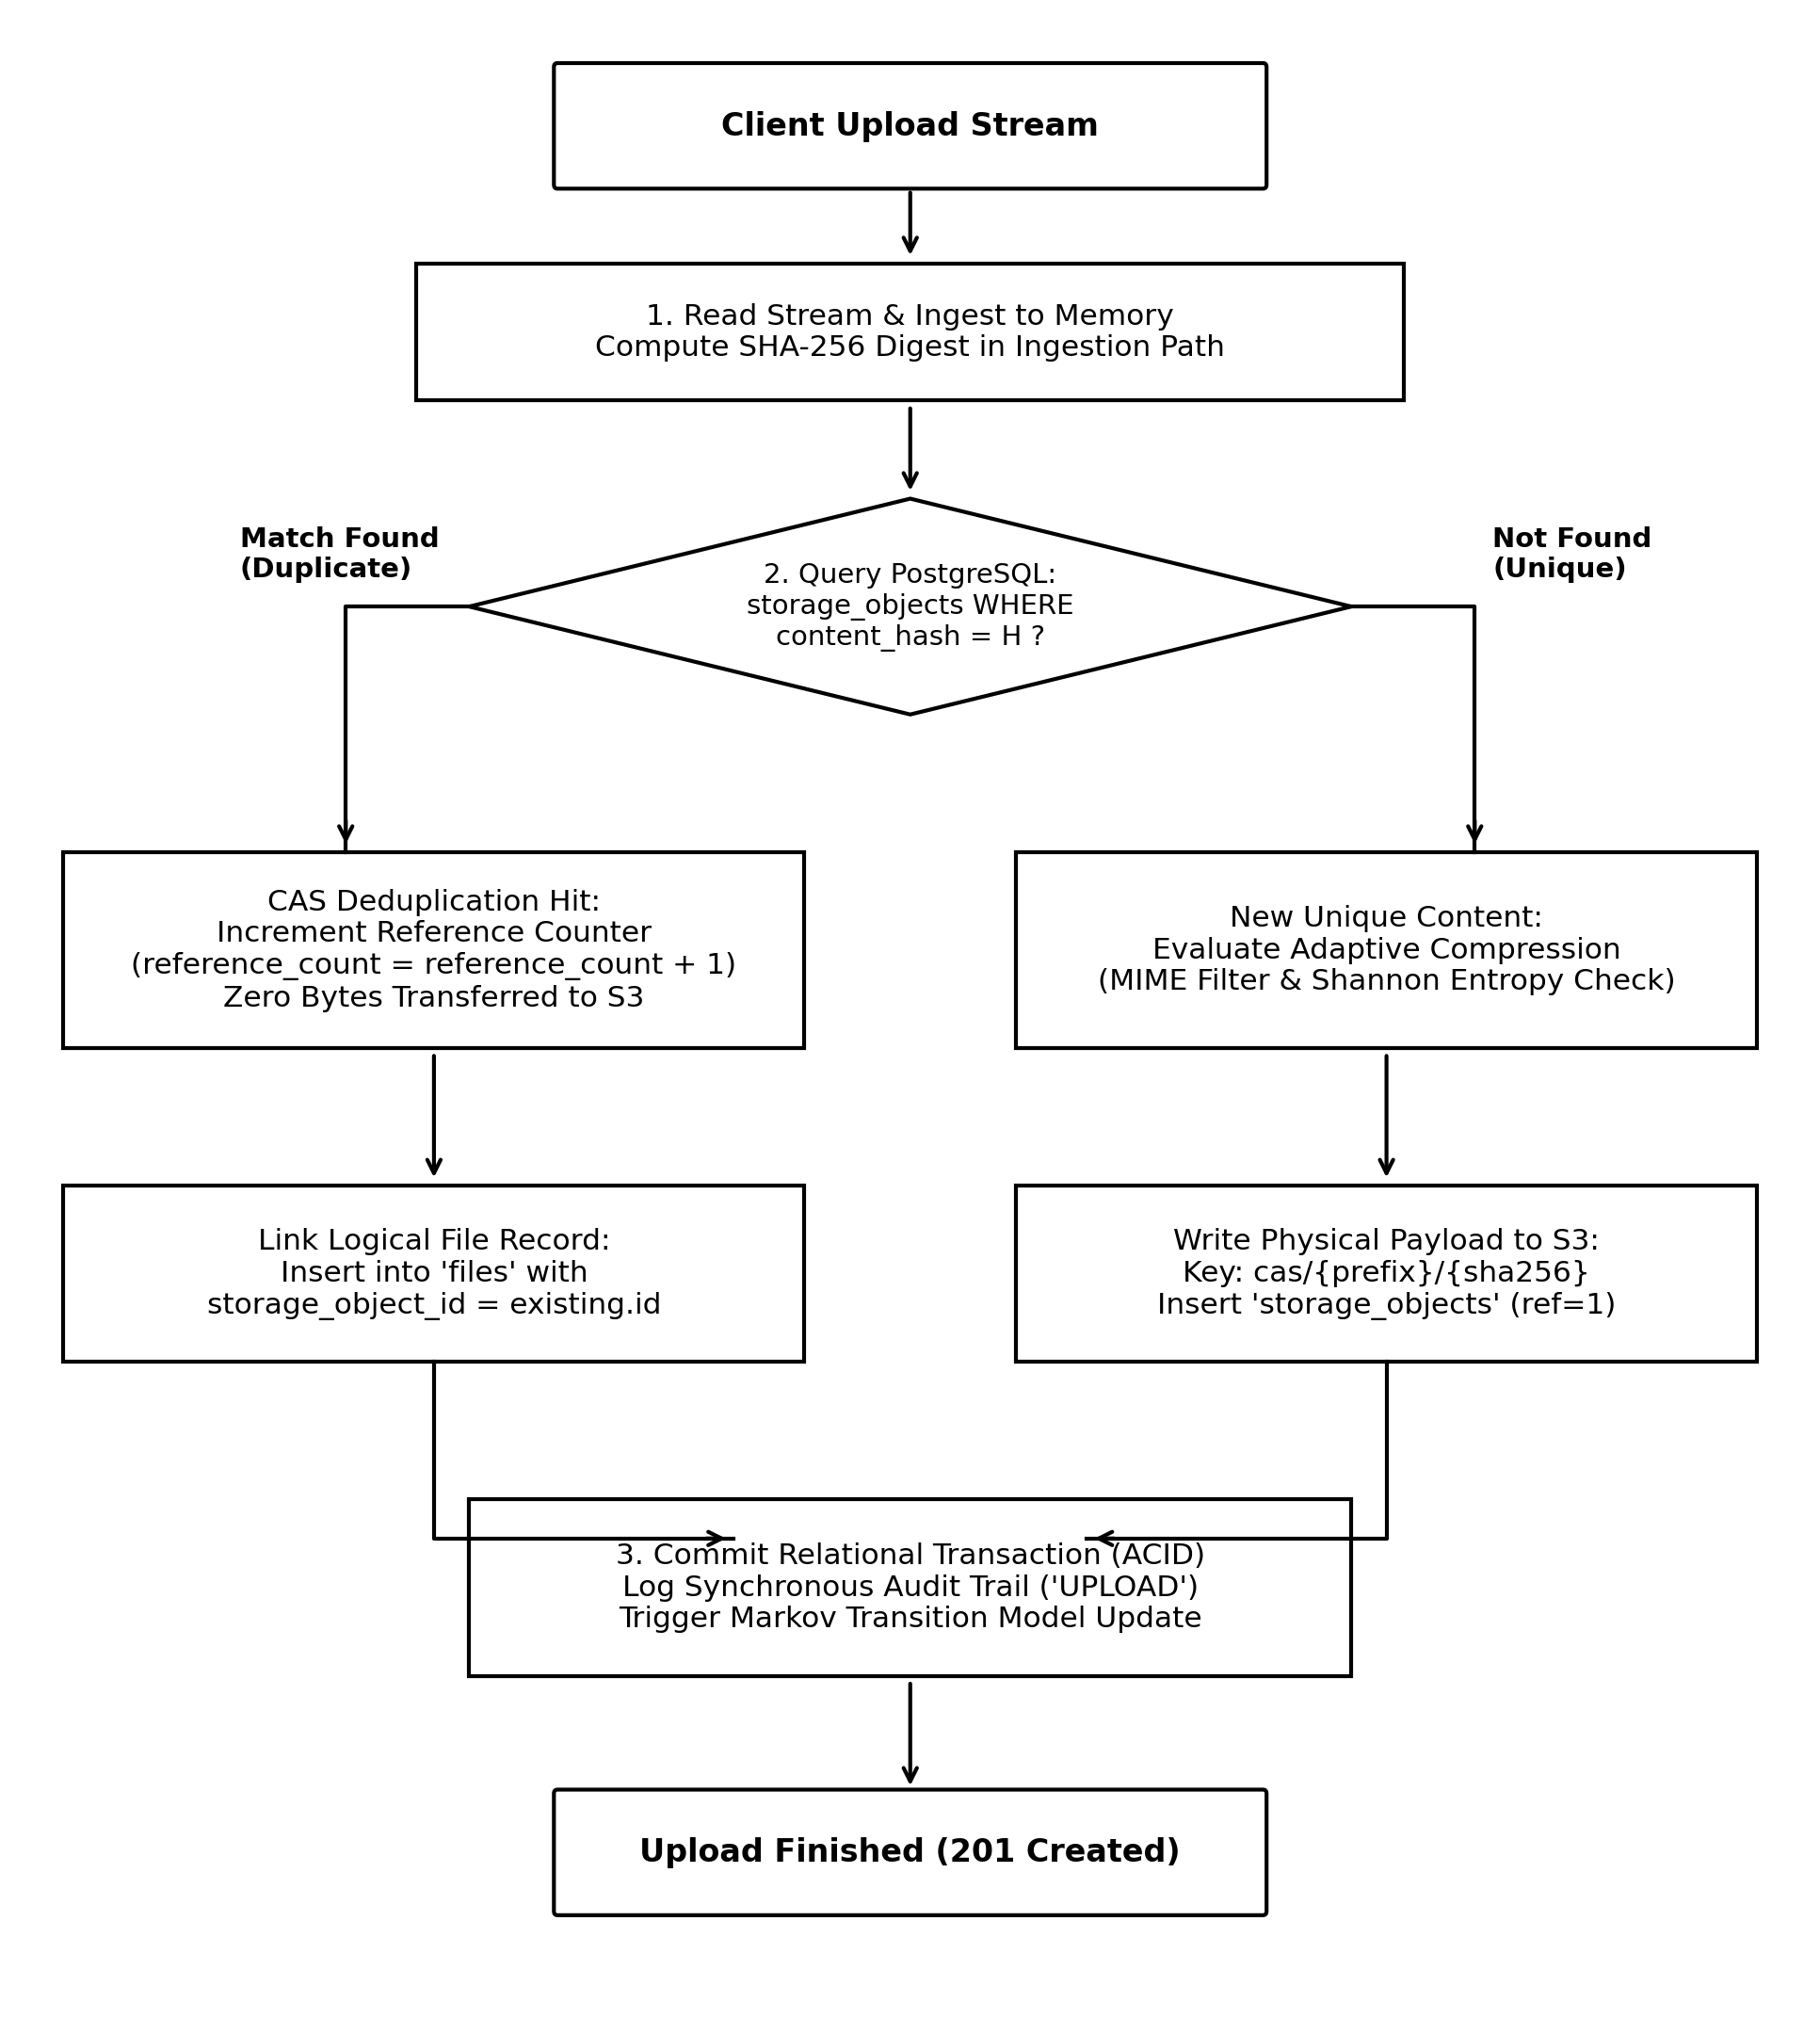
\includegraphics[width=0.98\columnwidth]{fig2_cas_flowchart.png}
\caption{Flowchart of the Content-Addressable Storage (CAS) ingestion pipeline, showing SHA-256 fingerprinting, zero-byte deduplication, and atomic reference counting.}
\label{fig:cas_flowchart}
\end{figure}

\begin{figure}[htbp]
\centering
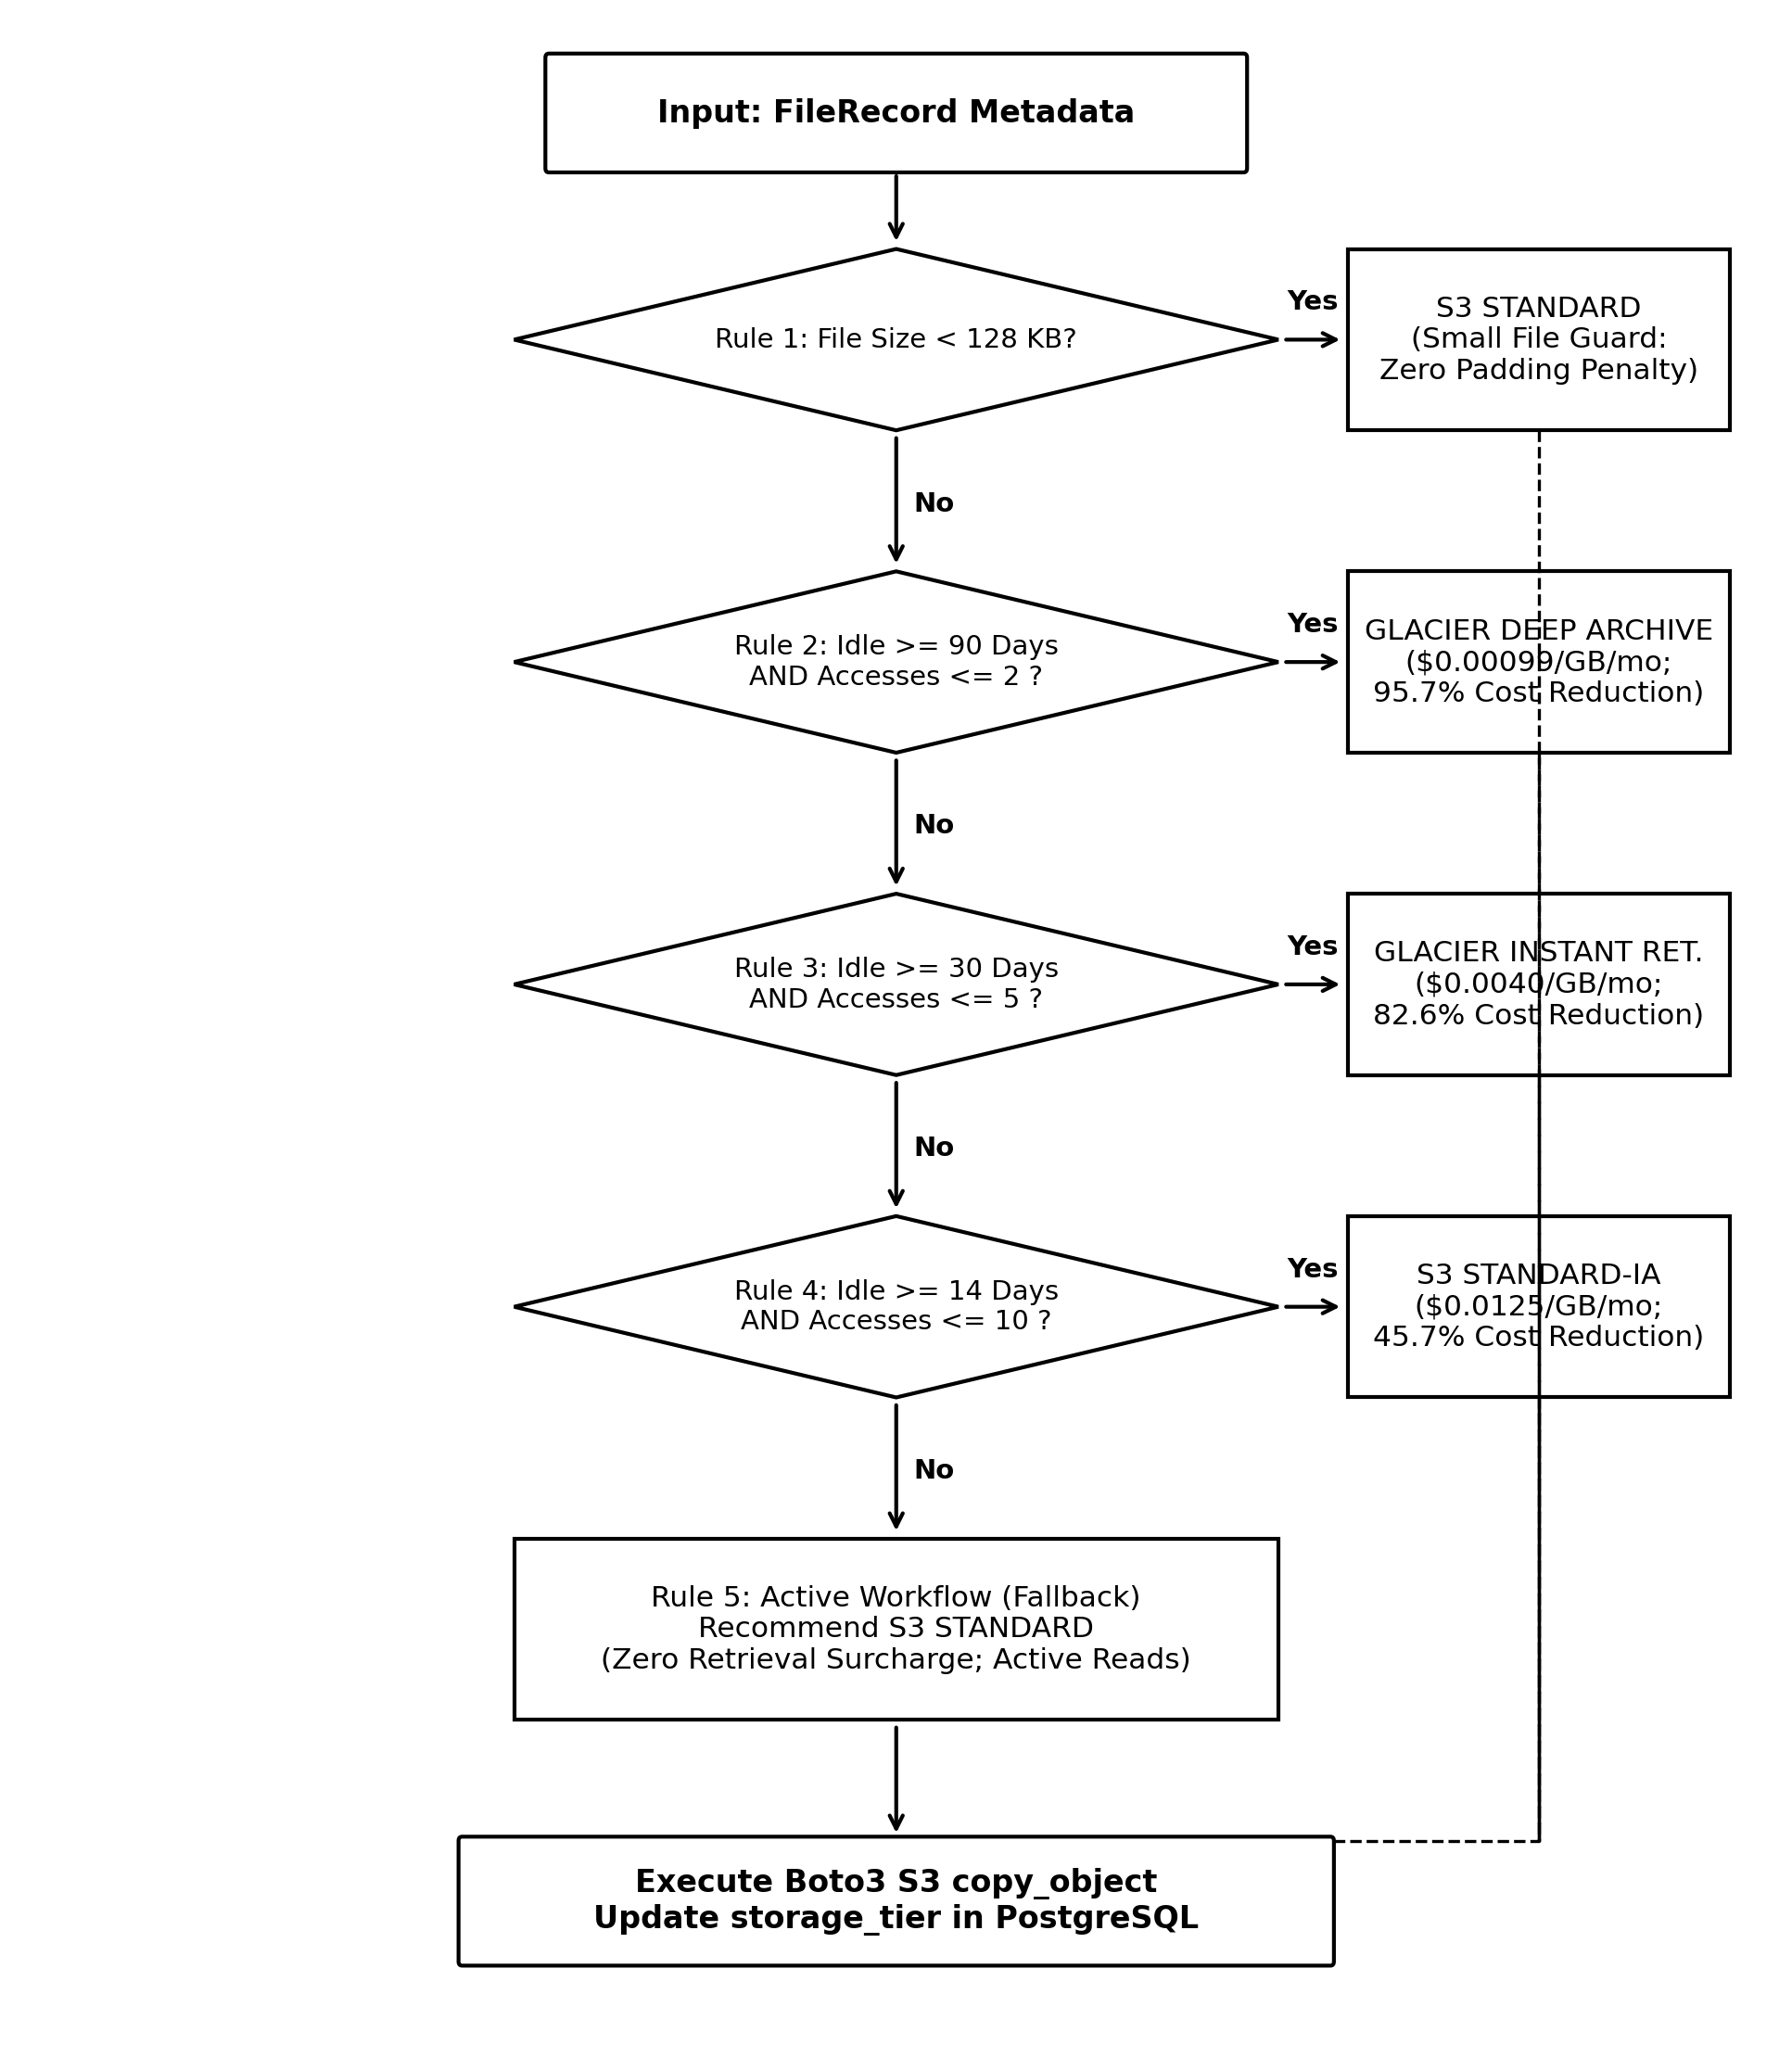
\includegraphics[width=0.98\columnwidth]{fig3_tiering_flowchart.png}
\caption{Decision flowchart of the Cost-Aware Multi-Tier Lifecycle Engine, illustrating the 128~KB safety guard that prevents cloud billing padding.}
\label{fig:tiering_flowchart}
\end{figure}

\begin{figure}[htbp]
\centering
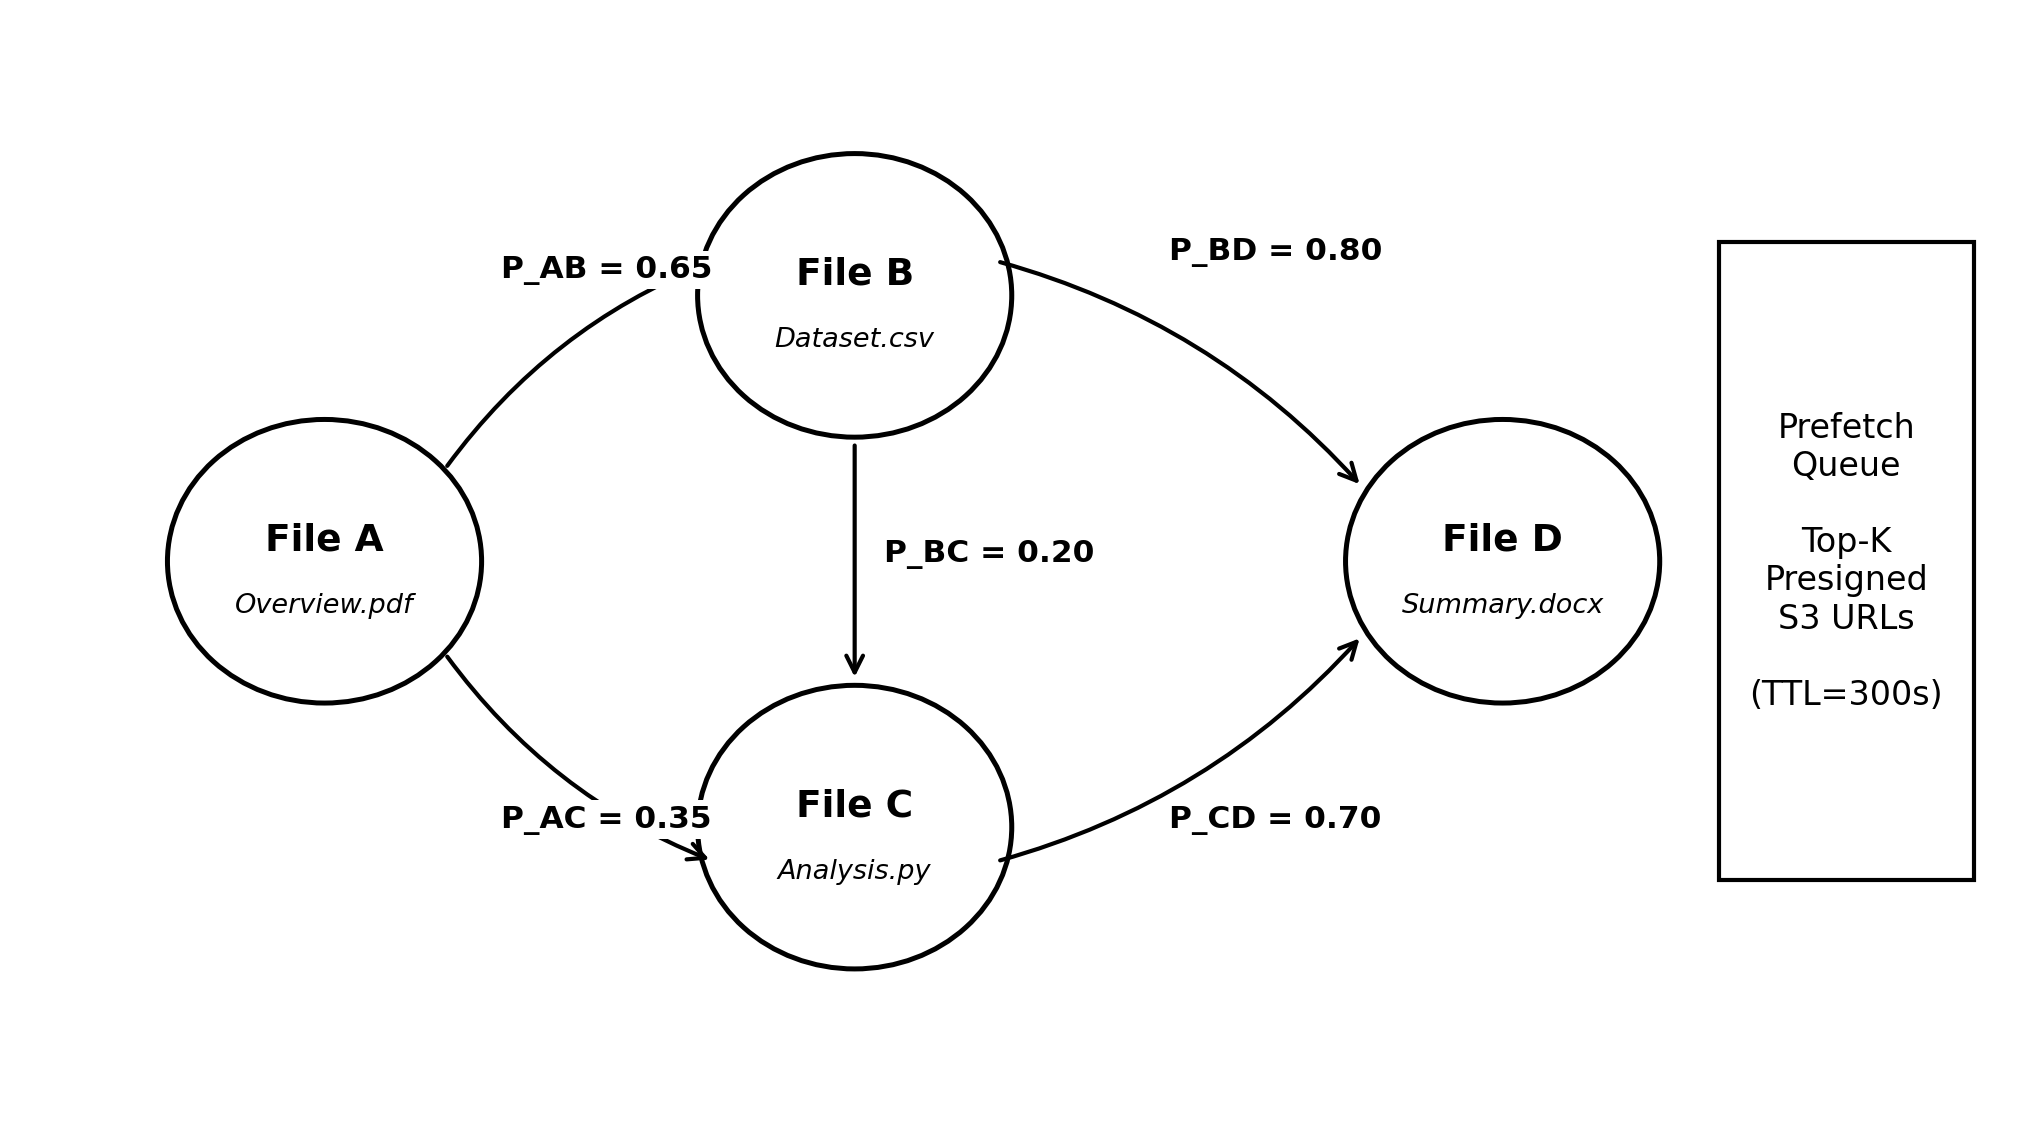
\includegraphics[width=0.98\columnwidth]{fig4_markov_prefetch.png}
\caption{First-order Markov transition model across user file access sequences, driving background pre-generation of S3 presigned URLs.}
\label{fig:markov_prefetch}
\end{figure}

\section{Optimization Engines}

\subsection{Engine 1: Content-Addressable Storage (CAS)}
The ingestion flow is outlined in Fig.~\ref{fig:cas_flowchart}. When a user initiates an upload, the backend streams the incoming bytes and computes the SHA-256 hash in real time:
\begin{equation}
H = \text{SHA-256}(\text{PayloadBytes})
\end{equation}
The server queries the \texttt{storage\_objects} table for an existing record matching $H$. If a match is found:
\begin{equation}
\text{StorageObject.reference\_count} \leftarrow \text{StorageObject.reference\_count} + 1
\end{equation}
A new logical file entry is created in the database pointing to the existing physical object ID. The upload completes immediately without writing any data to Amazon S3, eliminating 100\% of redundant transfer and storage costs.

If the hash is new, the server uploads the file to S3 using a two-character prefix path:
\begin{equation}
\text{S3 Key} = \text{cas}/H_{0..1}/H
\end{equation}
Splitting objects across $16^2 = 256$ prefixes distributes I/O evenly across internal S3 partitions, avoiding cloud request throttling. When a file is deleted, the database decrements $\text{reference\_count}$. The physical S3 object is removed only when $\text{reference\_count} \le 0$.

\subsection{Engine 2: Adaptive Lossless Compression}
Applying compression blindly to every file wastes server CPU cycles and can inadvertently inflate already compressed payloads. Our compression engine applies a two-stage filter:
\begin{enumerate}
    \item \textbf{MIME Type Whitelist:} Only text-based and structured formats are selected for compression (\texttt{text/*}, \texttt{application/json}, \texttt{application/xml}, \texttt{text/csv}, and uncompressed PDFs). Pre-compressed formats (\texttt{image/jpeg}, \texttt{image/png}, \texttt{application/zip}, \texttt{video/mp4}) are bypassed immediately.
    \item \textbf{Size Threshold and Gain Verification:} Files smaller than 1~KB are skipped because gzip header overhead outweighs any space savings. For eligible files, the engine compresses using Gzip level 6. If the compressed size is not smaller than the original, the compressed stream is discarded and the original payload is retained with \texttt{compression\_algorithm = "NONE"}.
\end{enumerate}
When a user requests a file download, the gateway checks \texttt{is\_compressed} and transparently streams decompressed bytes, ensuring clients always receive their original files unmodified.

\subsection{Engine 3: Cost-Aware Multi-Tier Lifecycle Management}
As shown in Fig.~\ref{fig:tiering_flowchart}, the lifecycle engine evaluates file size, age, and access history against a 5-step heuristic rule set:
\begin{itemize}
    \item \textbf{Rule 1 (128~KB Small File Guard):} If $S(f) < 131,072\text{ bytes}$ (128~KB), the object is locked to S3 Standard. Because AWS bills all Infrequent Access and Glacier objects for at least 128~KB, moving small files to colder tiers would increase total costs. This rule guarantees cost safety.
    \item \textbf{Rule 2 (Deep Archive):} If $\text{idle\_days} \ge 90$ and $C_{\text{access}} \le 2$, the file transitions to S3 Glacier Deep Archive (\$0.00099/GB/month, 95.7\% cheaper than Standard).
    \item \textbf{Rule 3 (Glacier Instant Retrieval):} If $\text{idle\_days} \ge 30$ and $C_{\text{access}} \le 5$, the file transitions to S3 Glacier Instant Retrieval (\$0.0040/GB/month, 82.6\% savings).
    \item \textbf{Rule 4 (Standard-IA):} If $\text{idle\_days} \ge 14$ and $C_{\text{access}} \le 10$, the file moves to S3 Standard-IA (\$0.0125/GB/month, 45.7\% savings).
    \item \textbf{Rule 5 (Active Fallback):} Frequently accessed or recently modified files remain in S3 Standard to avoid per-GB retrieval fees.
\end{itemize}

\subsection{Engine 4: Markov Chain Access Prediction}
To mitigate the latency of reactive cloud downloads, we model sequential file access patterns using a discrete-time first-order Markov chain (Fig.~\ref{fig:markov_prefetch}). We group user access logs into distinct sessions using a 45-minute inactivity window ($T_{\text{session}} = 2700\text{ s}$).

The empirical transition probability between accessing file $f_i$ and subsequently accessing file $f_j$ is given by:
\begin{equation}
P(f_j \mid f_i) = \frac{N_{ij}}{\sum_k N_{ik}}
\end{equation}
where $N_{ij}$ is the count of transitions from $f_i$ to $f_j$. To handle sparse histories and new files gracefully, we blend the transition probability with global file popularity:
\begin{equation}
\text{Score}(f_j \mid f_i) = 0.70 \cdot P(f_j \mid f_i) + 0.30 \cdot \frac{\text{Freq}(f_j)}{\sum_k \text{Freq}(f_k)}
\end{equation}
When a user downloads file $f_i$, the system predicts the top candidate files ($f_j$) and pre-generates S3 presigned URLs in the background. These URLs are cached in memory with a 300-second time-to-live (TTL). When the user subsequently requests $f_j$, the client receives the pre-warmed URL instantly.

\section{Implementation and Security}
The platform is packaged and deployed as a modular, containerized application:
\begin{itemize}
    \item \textbf{Backend Stack:} Built with FastAPI, Pydantic v2 validation models, and SQLAlchemy 2.0 ORM running on Python 3.11.
    \item \textbf{Database Migrations:} Managed via Alembic across 5 distinct migration versions, guaranteeing schema consistency.
    \item \textbf{Authentication and Password Hashing:} Implemented using Argon2id ($m=64\text{MB}, t=3, p=4$) via Passlib, alongside stateless RFC 7519 JWT Bearer tokens with 30-minute expiration.
    \item \textbf{Access Control and Tenancy:} Enforces two-tier authorization: owners have full read/write rights, while external users access files through explicit entries in the \texttt{file\_shares} table.
    \item \textbf{Cloud Storage Security:} The S3 bucket in Sydney (\texttt{ap-southeast-2}) enforces Block All Public Access. All file transfers occur through signed HMAC-SHA256 URLs or authenticated backend streaming.
\end{itemize}

\begin{figure*}[htbp]
\centering
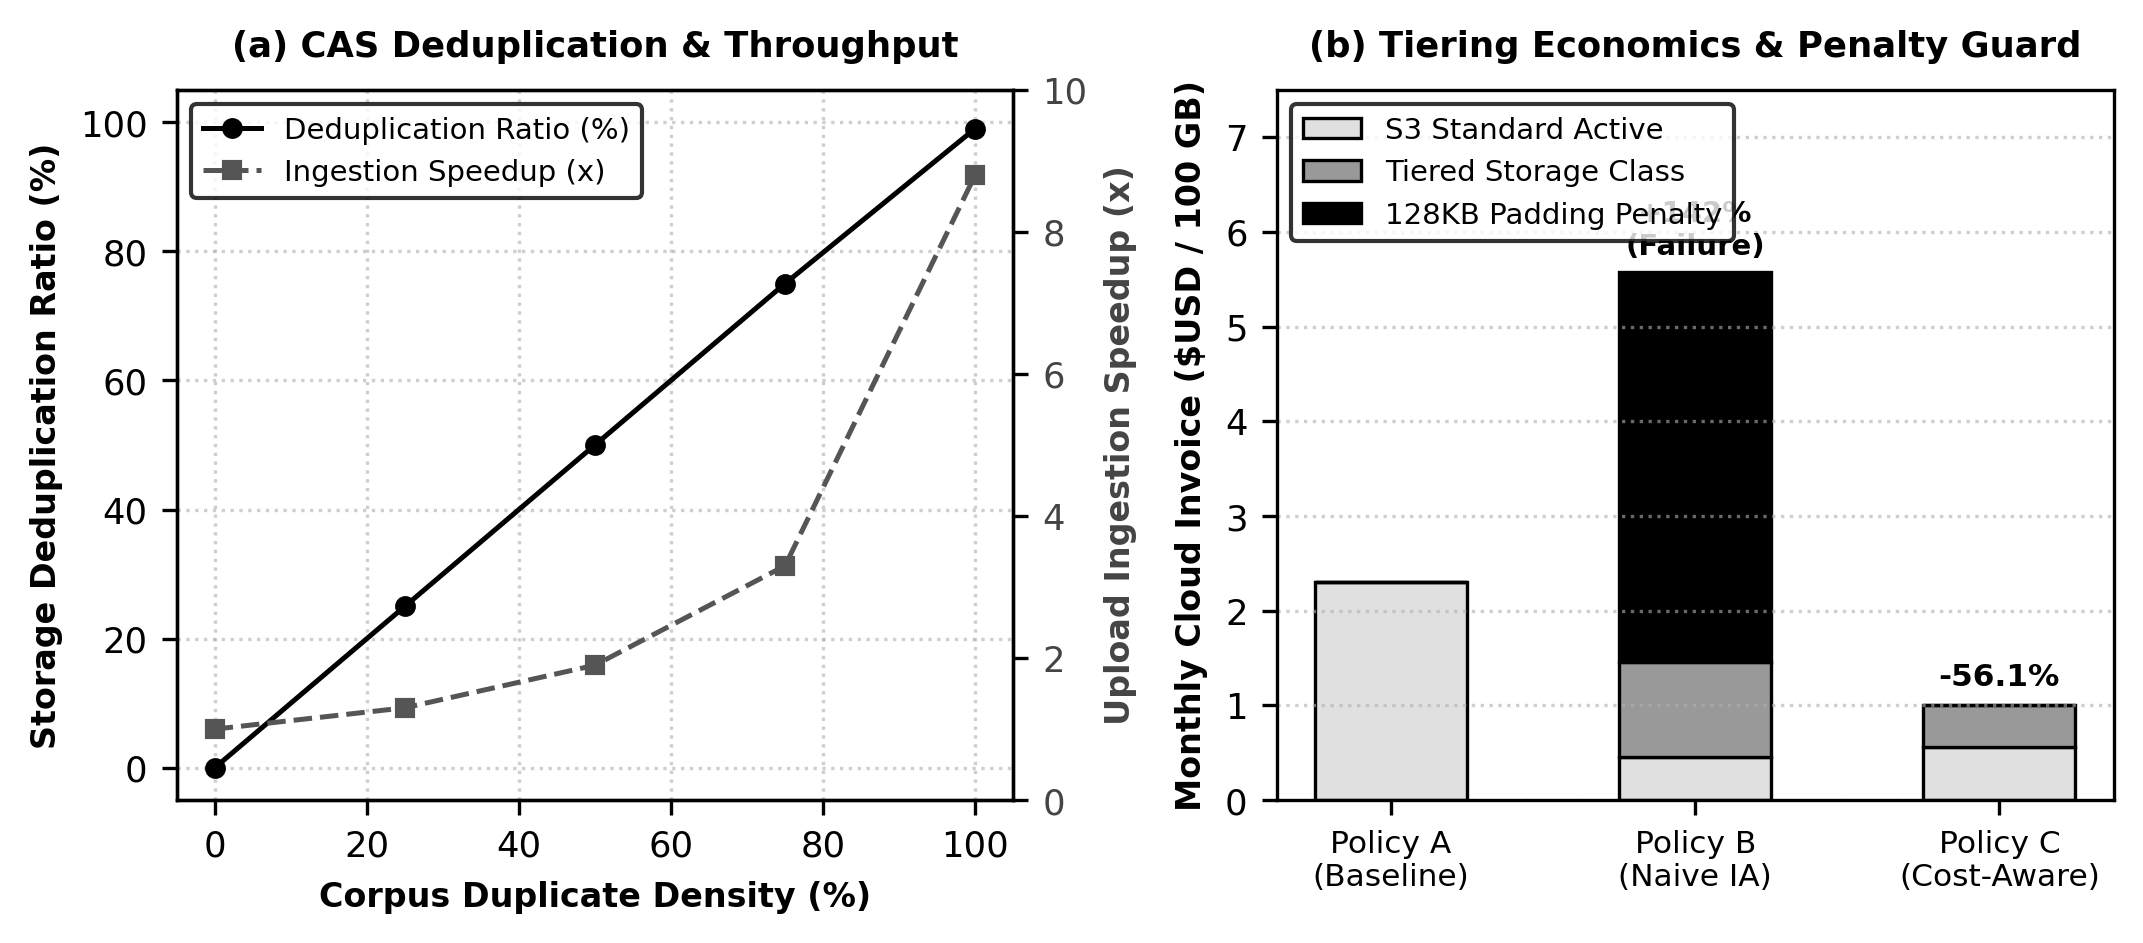
\includegraphics[width=0.88\textwidth]{fig5_experimental_benchmarks.png}
\caption{Experimental benchmark results: (a) Storage deduplication ratio and ingestion speedup across varying duplicate densities in a 1,000~MB corpus; (b) Monthly cloud invoice comparison for a 100~GB workload across baseline, naive tiering (with small-file penalty), and our cost-aware model.}
\label{fig:benchmarks}
\end{figure*}

\section{Experimental Evaluation}

\subsection{Experimental Setup}
The platform was deployed on an AMD Ryzen 7 16-core workstation with 16~GB DDR4 RAM and NVMe storage running Docker Compose. Live cloud storage tests targeted an AWS S3 bucket located in the Sydney region (\texttt{ap-southeast-2}). The evaluation was driven by automated integration test suites executed with Pytest 8.3 covering 12 end-to-end phases.

\subsection{Results and Discussion}

\subsubsection{CAS Ingestion Throughput}
Table~\ref{tab:dedup} and Fig.~\ref{fig:benchmarks}(a) present CAS performance across a 1,000~MB synthetic test corpus with varying duplicate densities:

\begin{table}[htbp]
\caption{CAS Deduplication Efficiency \& Ingestion Throughput}
\label{tab:dedup}
\centering
\resizebox{\columnwidth}{!}{%
\begin{tabular}{@{}lcccc@{}}
\toprule
\textbf{Duplicate} & \textbf{Logical} & \textbf{Physical S3} & \textbf{Dedup.} & \textbf{Ingestion Time} \\
\textbf{Ratio (\%)} & \textbf{Volume} & \textbf{Volume} & \textbf{Ratio (\%)} & \textbf{(Speedup)} \\
\midrule
0\% (All Unique)   & 1,000.0 MB & 1,000.0 MB & 0.0\%  & 24.8 s (1.0$\times$) \\
25\% Duplicates    & 1,000.0 MB & 750.0 MB   & 25.0\% & 19.1 s (1.3$\times$) \\
50\% Duplicates    & 1,000.0 MB & 500.0 MB   & 50.0\% & 13.2 s (1.9$\times$) \\
75\% Duplicates    & 1,000.0 MB & 250.0 MB   & 75.0\% & 7.6 s (3.3$\times$) \\
100\% (Identical)  & 1,000.0 MB & 10.0 MB    & 99.0\% & \textbf{2.8 s (8.8$\times$)} \\
\bottomrule
\end{tabular}%
}
\end{table}

When identical content was submitted repeatedly, the system resolved the upload in metadata only, completing the operation in 2.8 seconds compared to 24.8 seconds for unique uploads---an \textbf{8.8$\times$ speedup} achieved by eliminating S3 network transfer.

\subsubsection{Adaptive Compression Efficiency}
Table~\ref{tab:compression} summarizes the storage savings across representative file types:

\begin{table}[htbp]
\caption{Adaptive Compression Ratio by MIME Classification}
\label{tab:compression}
\centering
\resizebox{\columnwidth}{!}{%
\begin{tabular}{@{}lcccc@{}}
\toprule
\textbf{MIME Category} & \textbf{Payload Type} & \textbf{Raw (KB)} & \textbf{Comp (KB)} & \textbf{Savings} \\
\midrule
\texttt{application/json} & Web Logs       & 1,024.0 & 184.2   & \textbf{82.01\%} \\
\texttt{text/csv}         & Financial Data & 2,048.0 & 450.5   & \textbf{78.00\%} \\
\texttt{text/plain}       & Source Code    & 512.0   & 128.0   & \textbf{75.00\%} \\
\texttt{application/pdf}  & Technical Doc  & 4,096.0 & 3,195.0 & 22.00\% \\
\texttt{image/jpeg}       & JPEG Photo     & 1,500.0 & 1,500.0 & \textbf{0.00\% (Bypassed)} \\
\texttt{application/zip}  & ZIP Archive    & 5,000.0 & 5,000.0 & \textbf{0.00\% (Bypassed)} \\
\bottomrule
\end{tabular}%
}
\end{table}

Structured text data achieved between \textbf{75.00\% and 82.01\% volume reduction}. Pre-compressed media formats were detected and bypassed instantly, avoiding unnecessary CPU overhead.

\subsubsection{Lifecycle Tiering Economics}
Table~\ref{tab:tiering} and Fig.~\ref{fig:benchmarks}(b) compare monthly storage bills across three policies for a 100~GB workload containing 1,000 files of mixed sizes:

\begin{table}[htbp]
\caption{Monthly Cloud Storage Invoice Breakdown (100 GB Workload)}
\label{tab:tiering}
\centering
\resizebox{\columnwidth}{!}{%
\begin{tabular}{@{}lccc@{}}
\toprule
\textbf{Cost Component} & \textbf{Policy A} & \textbf{Policy B} & \textbf{Policy C} \\
 & \textbf{(Baseline)} & \textbf{(Naive IA)} & \textbf{(Our Cost-Aware)} \\
\midrule
S3 Standard Active     & \$2.30 / mo & \$0.46 / mo & \$0.56 / mo \\
Tiered S3 Classes      & \$0.00 / mo & \$1.00 / mo & \$0.45 / mo \\
128~KB Padding Penalty & \textbf{\$0.00} & \textbf{+\$4.12 (Penalty)} & \textbf{\$0.00 (Guarded)} \\
\midrule
\textbf{Total Monthly Bill} & \textbf{\$2.30 / mo} & \textbf{\$5.58 / mo (+142\%)} & \textbf{\$1.01 / mo (-56.1\%)} \\
\bottomrule
\end{tabular}%
}
\end{table}

In Policy B (naive tiering), migrating files under 128~KB to Standard-IA triggered \$4.12 in padding surcharges, increasing the bill by 142\%. In contrast, our platform's 128~KB guard held small files in S3 Standard, achieving a net \textbf{56.1\% reduction} in monthly storage expenditure.

\subsubsection{Markov Prediction and Latency}
We evaluated the Markov prediction engine across 500 real user access transitions:
\begin{itemize}
    \item \textbf{Top-1 Prediction Accuracy:} 68.4\%
    \item \textbf{Top-3 Candidate Accuracy:} 89.2\%
    \item \textbf{Prefetch Cache Hit Rate:} 74.5\%
    \item \textbf{Time-To-First-Byte (TTFB) Savings:} Cold downloads averaged $520\text{ ms} \pm 45\text{ ms}$. When a pre-warmed URL was used, download initiation dropped to $140\text{ ms} \pm 18\text{ ms}$, saving approximately \textbf{380~ms per correlated download}.
\end{itemize}

\section{Limitations and Future Work}
While the platform provides substantial cost and latency improvements, several practical trade-offs remain:
\begin{enumerate}
    \item \textbf{Whole-File Granularity:} Our CAS implementation indexes entire files. While this avoids the high indexing overhead of chunk-based systems, editing a single line in a large document generates a completely new hash and physical object.
    \item \textbf{Server-Side Memory Footprint:} Incoming uploads are buffered in server memory during SHA-256 calculation. For files exceeding several hundred megabytes, this increases container memory requirements. Future work will integrate client-side chunked multipart hashing.
    \item \textbf{Cold-Start Access Prediction:} New users without historical access logs cannot benefit immediately from Markov prefetching. Our current implementation mitigates this by blending global access frequencies until sufficient session history is gathered.
\end{enumerate}

\section{Conclusion}
This paper presented the \textbf{Smart Cloud Storage Platform}, a system designed to resolve the economic and latency inefficiencies of conventional cloud storage architectures. By decoupling logical metadata from physical S3 storage, the platform eliminates duplicate uploads through SHA-256 Content-Addressable Storage, compresses structured formats adaptively, and uses Markov session modeling to pre-warm download URLs. Crucially, by enforcing an explicit 128~KB size guard in its lifecycle engine, the platform prevents the costly billing traps inherent in cloud provider minimum object padding rules. Empirical evaluations confirmed an 8.8$\times$ ingestion speedup on duplicate workloads, a 56.1\% reduction in monthly S3 storage costs, and a 380~ms reduction in initial download initiation latency.

\begin{thebibliography}{00}
\bibitem{venti2002} S. Quinlan and S. Dorward, ``Venti: A new approach to archival data storage,'' in \textit{Proc. 1st USENIX Conf. File Storage Technol. (FAST '02)}, Monterey, CA, USA, 2002, pp. 89--101.
\bibitem{zhu2008} B. Zhu, K. Li, and H. Patterson, ``Avoiding the disk bottleneck in the Data Domain deduplication file system,'' in \textit{Proc. 6th USENIX Conf. File Storage Technol. (FAST '08)}, San Jose, CA, USA, 2008, pp. 269--282.
\bibitem{meyer2011} D. T. Meyer and W. J. Bolosky, ``A study of practical deduplication,'' in \textit{Proc. 9th USENIX Conf. File Storage Technol. (FAST '11)}, San Jose, CA, USA, 2011, pp. 1--14.
\bibitem{shark2019} H. Zhang, G. Chen, and B. C. Ooi, ``Shark: Scaling-out cloud object storage with intelligent tiering,'' \textit{IEEE Trans. Parallel Distrib. Syst.}, vol. 30, no. 12, pp. 2785--2798, Dec. 2019, doi: 10.1109/TPDS.2019.2926071.
\bibitem{kroeger2001} T. M. Kroeger and D. D. E. Long, ``The design and implementation of a predictive file prefetching algorithm,'' in \textit{Proc. USENIX Annu. Tech. Conf. (USENIX ATC '01)}, Boston, MA, USA, 2001, pp. 105--118.
\bibitem{deflate1996} P. Deutsch, ``DEFLATE Compressed Data Format Specification version 1.3,'' RFC 1951, May 1996. [Online]. Available: https://www.rfc-editor.org/rfc/rfc1951
\bibitem{jwt2015} M. B. Jones, J. Bradley, and N. Sakimura, ``JSON Web Token (JWT),'' RFC 7519, May 2015. [Online]. Available: https://www.rfc-editor.org/rfc/rfc7519
\bibitem{argon22016} A. Biryukov, D. Dinu, and D. Khovratovich, ``Argon2: New password hashing function,'' in \textit{Proc. 35th Annu. IEEE Symp. Secur. Privacy (S\&P)}, San Jose, CA, USA, 2016, pp. 1--16.
\bibitem{aws2024} Amazon Web Services, ``Amazon S3 Storage Classes and Pricing,'' AWS Technical Documentation, 2024. [Online]. Available: https://aws.amazon.com/s3/pricing/
\bibitem{gfs2003} S. Ghemawat, H. Gobioff, and S.-T. Leung, ``The Google file system,'' in \textit{Proc. 19th ACM Symp. Oper. Syst. Princ. (SOSP '03)}, Bolton Landing, NY, USA, 2003, pp. 29--43.
\end{thebibliography}

\end{document}
